\documentclass{article}

\usepackage[tmargin=1in,bmargin=1in,lmargin=1.25in,rmargin=1.25in]{geometry}
\usepackage{graphicx}
\usepackage{hyperref}
\usepackage{amsmath}

\thispagestyle{empty}

\begin{document}


\title{ \normalsize \textsc{}
	\\ [2.0cm]
%	\HRule{1.5pt} \\
	\Large \textbf{\uppercase{Optimizing a High-Dimension Compartment ODE Model}
}
}
\date{December 2023}
\author{Jeremy Chiu,\\APMA 923, Dr. JF Williams} 
	

\maketitle
%\newpage
%\tableofcontents

\section{Project Overview}

We consider the compartment ODE model presented by Guo-Wu\cite{GuoWu}, which describes the spread of Tuberculosis (TB) among the Canadian foreign-born population.  Their ODE model is includes 5 dependent variables and 9 parameters, some of which are difficult to measure or estimate.  Our goal is to find the parameters that give the global minimum of the model's prediction error (by comparing model output to real-world reported data).

\subsection{Background and loss function}


We consider the compartment ODE model presented by Guo-Wu\cite{GuoWu}, which describes the spread of Tuberculosis (TB) among the Canadian foreign-born population.  Fundamentally, an SEIR-model is used, where the \textit{exposed} category is partitioned into \textit{early latent} and \textit{late latent}.  Figure \ref{fig:flow} shows a flow diagram of their model.

\begin{figure}
		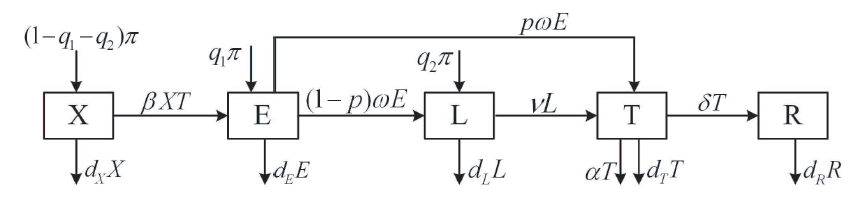
\includegraphics[scale=0.4]{xeltr flow diagram}
		\caption{Flow diagram of the compartment ODE model used by \cite{GuoWu}.}
		\label{fig:flow}
\end{figure}

After fixing initial conditions and parameter values, we use Matlab's \texttt{ode23} routine to solve the system of differential equations from \cite{GuoWu}, which returns population vs time.  From the population, we compute the TB incidence
$$\text{Estimated TB Incidence } = \frac{100,000}{X(t)+E(t)+L(t)+T(t)+R(t)} \cdot (pw E(t) + v L(t)) ,$$
which can be compared to the reported TB incidence from Canadian reports\cite{MounchiliA.2022TuberculosisReport} (see figure \ref{fig:foreignBornData}).  The error is defined to be the difference between our computed (estimated) incidence and the reported incidence.  We use parameters that are difficult to measure as input to the optimizer: $q_1$ and $q_2$ are the percentage of new immigrants that are undetected by Canadian TB screening, and the initial populations $E_0$, $L_0$, and $R_0$ are unknown; for a total of 5 variables to optimize across.  Note that $T_0$ is reported, and $X_0$ is computed from the reported total foreign-born population, and all other parameters use estimates found from a literature search.

\begin{figure}
	\centering 
	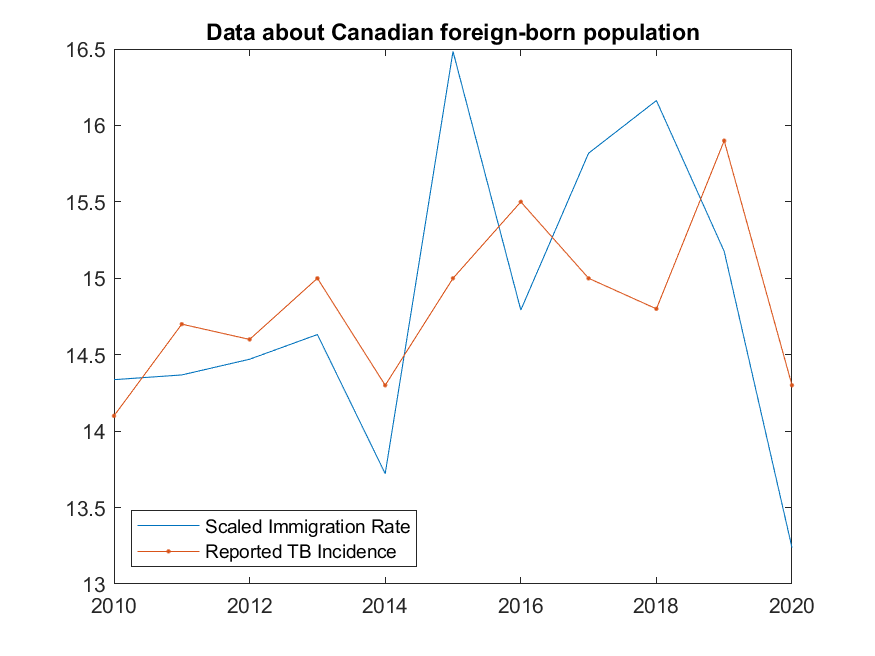
\includegraphics[scale=0.6]{foreignBornData}
	\caption{Reported incidence of Canadian foreign-born population.  Annual immigration rate is also presented, scaled to be on same viewing rectangle.  Notice how the number of immigrants drive the incidence rate.}
	\label{fig:foreignBornData}
\end{figure}


	\subsection{Project Proposal Meeting}
	
	JF and I met on October 27 to discuss the project.  Here were JF's suggestions about possible things to try:
	
	\begin{itemize}
		\item Do not over expand on problem background.  Discuss how we solved it.
		\item Compare solvers.
		\item Try to find local sensitivity.  Investigate derivatives with respect to parameters.
		\item Discuss \texttt{fmincon}.
		\item Global optimization toolbox.
		\item Find an upper bound on $q_1$ and $q_2$ using immigration data.
		\item Investigate convexity.
	\end{itemize}

	\section{Finding the global min with \texttt{fmincon}}

	We used Matlab's constrained solver, \texttt{fmincon}.  Our constraints were 
	$$ q_1,~q_2,~E_0,~L_0,~R_0 \geq 0, \text{ and } q_1+q_2 \leq 1$$
	Initial conditions were the original proportions presented in \cite{GuoWu}.  The solver does a decent job in minimization -- figure \ref{fig:optimizedIncidence} shows the estimated incidence after optimization, which is reasonably close to the reported incidence.
	
	\begin{figure}
		\centering 
		\includegraphics[scale=0.6]{{PopVsTime_optimized}}
		\caption{After optimization, the model reasonably estimate incidence.}
		\label{fig:optimizedIncidence}
	\end{figure}
	
	\subsection{Sensitivity Analysis}
	
	
	
	
	\section{Future Work}
	
	something I tried:
		--  freeze thaw -- optimize across $q_1$, $q_2$, and $E_0$, THEN $L_0$





\bibliographystyle{plain} % We choose the "plain" reference style
\bibliography{tb-bib}


\end{document}
